\section{Metodologia}
Esta sección describe detalladamente el procedimiento metodológico aplicado
para construir y resolver el modelo numérico de intercepción de dos objetivos
con un solo impulso, empleando métodos numéricos revisados y no revisados en
clase. El enfoque incluye la recolección y análisis de datos, el desarrollo del
algoritmo, la justificación metodológica y la identificación de limitaciones
del modelo.

\subsection{Recolección de datos}
Los datos utilizados para construir el modelo provienen de la Tabla 1 del
artículo de Xia et al. (2021), la cual define los elementos orbitales de tres
cuerpos: una nave perseguidora (S0) y dos objetivos (S1 y S2). Estos elementos
fueron introducidos en el modelo bajo el marco de un sistema de dos cuerpos,
tal como se planteó anteriormente.

Las herramientas y software utilizados se listan a continuación:

\begin{itemize}
    \item MATLAB, para la implementación computacional del modelo
    \item Funciones propias en MATLAB para la conversión de elementos orbitales,
          propagación de trayectorias, cálculo de anomalías y generación de Porkchop
          plots.
    \item Scripts adaptados para aplicar el método de Gibbs y resolver sistemas no
          lineales con Newton-Raphson
\end{itemize}

\subsection{Análisis de datos}
Se desarrolló un proceso iterativo compuesto por las siguientes etapas:

\subsubsection{Conversión de elementos orbitales}
A partir de los valores de periapsis $rp$ y apoapsis $ra$, se calculó el
semieje mayor $a$ y la excentricidad $e$ de acuerdo a las siguientes fórmulas:

\begin{itemize}
    \item $a = (rp + ra) / 2$
    \item $e = \frac{ra - rp}{ra + rp}$
\end{itemize}

\subsubsection{Transformación a vectores de estado}
Los elementos orbitales se convirtieron a vectores de posición y velocidad en
el sistema de coordenadas inerciales (ECI) usando funciones orbitales
conocidas.

\subsubsection{Generación de Porkchop plot}
Se exploró el espacio de tiempos de impulso $t_0$ e intercepción $t_1$ mediante
un Porkchop plot, evaluando la siguiente función para cada combinación:

$P = \left| t_1 - t_0 - \frac{M_{3, t_1} - M_{3, t_0}}{n_3} \right| + \left| t_2 - t_0 - \frac{M_{3, t_2} - M_{3, t_0}}{n_3} \right|$

Esto permitió seleccionar pares iniciales con valores mínimos de P como
candidatos para el método de Newton-Raphson \parencite{Wang2025}.

\subsubsection{Cálculo de t\textsubscript{2}}
A partir de los parámetros de $S_2$, se estimó $t_2$ utilizando la propagación
de la anomalía media para el segundo objetivo:

$t_2 = \frac{M_{2, t_2} - M_{2,t_i}}{n_2}$

\subsubsection{Método de Gibbs}
Con los vectores de posición $r_0$, $r_1$, y $r_2$, se utilizó el método de
Gibbs para calcular el vector de velocidad orbital de la nave perseguidora:

$v_{3, t_k} = \sqrt{\frac{\mu}{ND}} \left( \frac{\textbf{D} \times \textbf{r}_{3, t_k}}{r_{3, t_k}} + \textbf{S} \right)$

\subsubsection{Formulación de sistema no lineal}
Se planteó el siguiente sistema con las ecuaciones (3) y (4)

\begin{equation}
    \begin{cases}
        Q_1 = t_1 - t_0 = \dfrac{M_{3, t_1} - M_{3, t_0}}{n_3} \\
        Q_2 = t_2 - t_0 = \dfrac{M_{3, t_2} - M_{3, t_0}}{n_3}
    \end{cases}
\end{equation}

\subsubsection{Resolución con Newton-Raphson}
Se resolvió el sistema anterior usando el método de Newton-Raphson con
derivadas parciales analíticas en las variables $t_0$ y $t_1$ con una
tolerancia de $10e^{-5}$.

\subsubsection{Validación de resultados}
Se verificó la convergencia numérica y se graficaron las trayectorias de las
tres naves, confirmando intercepciones visuales con $S_1$ y $S_2$.

\subsection{Algoritmo}

A continuación, se presenta la serie de pasos a seguir para aplicar el método
al problema formulado:

\begin{enumerate}
    \item Cargar datos orbitales de S0, S1 y S2.
    \item Calcular $a$ y $e$ para cada cuerpo.
    \item Transformar elementos orbitales a vectores $(\mathbf{r}, \mathbf{v})$.
    \item Crear matriz de tiempos $t_0$, $t_1$ $\rightarrow$ Porkchop plot:
          \begin{enumerate}
              \item Calcular $t_2$ a partir de $M_2$ y $n_2$.
              \item Calcular error $P(t_0, t_1)$.
          \end{enumerate}
    \item Seleccionar pares con menor $P$ como estimaciones iniciales.
    \item Para cada par seleccionado:
          \begin{enumerate}
              \item Calcular $\mathbf{r}_0$, $\mathbf{r}_1$, $\mathbf{r}_2$.
              \item Calcular $\mathbf{v}$ mediante método de Gibbs.
              \item Determinar $M_3$ en $t_0$, $t_1$, $t_2$ y $n_3$.
              \item Resolver sistema no lineal con Newton-Raphson.
              \item Evaluar convergencia y guardar solución.
          \end{enumerate}
    \item Visualizar trayectorias y validar intercepciones.
\end{enumerate}

\subsection{Diagrama de flujo}

\begin{figure}[H]
    \centering
    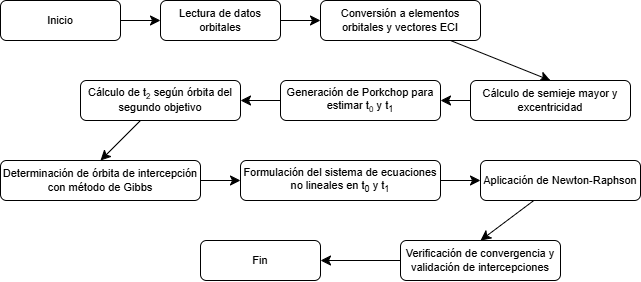
\includegraphics[width=0.9\textwidth]{flowchart.png}
    \caption{Diagrama de flujo del algoritmo propuesto.}
    \label{fig:flowchart}
\end{figure}

\newpage

\subsection{Justificación de método}
\begin{itemize}
    \item \textbf{Newton-Raphson}: Su velocidad de convergencia y precisión lo hacen adecuado para resolver sistemas no lineales con pocas variables, como el planteado.
    \item \textbf{Gibbs}: Permite estimar la velocidad orbital de una nave a partir de tres vectores de posición sin necesidad de integrar ecuaciones diferenciales.
    \item \textbf{Porkchop plot}: Nos permite explorar las combinaciones de tiempos de impulso e intercepción, optimizando la elección de valores iniciales.
\end{itemize}

\subsection{Limitaciones del enfoque}

\begin{enumerate}
    \item El modelo no considera perturbaciones como el término J2, lo que puede generar
          desviaciones en escenarios reales prolongados, o órbitas en las que el cuerpo
          central tiene una topología altamente irregular.

    \item La velocidad de convergencia de Newton-Raphson depende de las condiciones
          iniciales; elecciones pobres pueden generar fallas.

    \item Por otro lado, Gibbs requiere que los vectores de posición no sean colineales,
          lo que puede limitar su uso en situaciones particulares.
\end{enumerate}

